%!TEX program = pdflatex
\documentclass{tufte-handout}

%\geometry{showframe}% for debugging purposes -- displays the margins

\usepackage{amsmath}

% Set up the images/graphics package
\usepackage{graphicx}
\setkeys{Gin}{width=\linewidth,totalheight=\textheight,keepaspectratio}
\graphicspath{{graphics/}}

\title{Glycogen Metabolism}
\author{}
\date{}  % if the \date{} command is left out, the current date will be used

% The following package makes prettier tables.  We're all about the bling!
\usepackage{booktabs}

% The units package provides nice, non-stacked fractions and better spacing
% for units.
\usepackage{units}

% The fancyvrb package lets us customize the formatting of verbatim
% environments.  We use a slightly smaller font.
\usepackage{fancyvrb}
\fvset{fontsize=\normalsize}

% Small sections of multiple columns
\usepackage{multicol}

% Provides paragraphs of dummy text
\usepackage{lipsum}

% These commands are used to pretty-print LaTeX commands
\newcommand{\doccmd}[1]{\texttt{\textbackslash#1}}% command name -- adds backslash automatically
\newcommand{\docopt}[1]{\ensuremath{\langle}\textrm{\textit{#1}}\ensuremath{\rangle}}% optional command argument
\newcommand{\docarg}[1]{\textrm{\textit{#1}}}% (required) command argument
\newenvironment{docspec}{\begin{quote}\noindent}{\end{quote}}% command specification environment
\newcommand{\docenv}[1]{\textsf{#1}}% environment name
\newcommand{\docpkg}[1]{\texttt{#1}}% package name
\newcommand{\doccls}[1]{\texttt{#1}}% document class name
\newcommand{\docclsopt}[1]{\texttt{#1}}% document class option name

\begin{document}

\maketitle% this prints the handout title, author, and date

\begin{abstract}
\noindent Glycogen is an important storage macromolecule.  While we injest polysaccharides in a variety of forms, glycogen is the major carboydrate storage form in mammals.  This unit will cover the roles of glycogen, and how intracellular and extracellular signals result in glycogen synthesis or release.  Finally we will discuss the consequences of abberant glycogen storage.  For more details on this topic, we recommend \citet{Bollen1998} and chapter 11 of Lippincott's Illustrated Reviews: Biochemistry\cite{Ferrier2017}.
\end{abstract}

\tableofcontents
\pagebreak
\section{Learning Objectives}

\begin{itemize}
\item Evaluate how the structure of glycogen allows for compact but accessible storage of glucose molecules.
\item Understand how glycogen synthesis and glycolysis are regulated by intracellular metabolites.
\item Explain how protein phosphorylation regulates Glycogen Synthase and Glycogen Phosphorylase activities and how extracellular signals affect glycogen metabolism.
\item Assess the tissue-specific roles of insulin, adrenaline and glucagon in glycogen storage.
\item Distinguish between the functions of glycogen in liver, adipose and muscle and evaluate how alterations in glycogen metabolism affect the physiological functions of these tissues.
\item Explain how glycogen storage diseases can occur and how specific genes result in different pathophysiologies depending on both the gene, and tissue where it is expressed.
\end{itemize}

\section{Key Concepts and Vocabulary}

\begin{itemize}
	\item Glycogenesis
	\item Glycogenolysis
	\item Protein Phosphorylation
	\item Allosteric Regulation
	\item Adrenergic Signaling
	\item Branch Points
	\item Inborn Errors of Metabolism
\end{itemize}

\section{Structure and function of glycogen}

Glycogen is a homopolymer of glucose units connected to each other by $\alpha$1-4 or $\alpha$1-6 glycosidic linkages\sidenote{This nomenclature refers to a link between the \#1 position of one molecule of glucose (the anomeric carbon) and either the \#4 or the \#6 position on the next glucose.}.  This allows for many molecules of glucose to be compactly stored in the cell, and then made available upon energy or glucose demand.  A series of $\alpha$1-4 bonds result in a more or less straight chain of glucose molecules, while a $\alpha$1-6 linkage results in a branch point.  A single glucose monomer can have both a $\alpha$1-4 and $\alpha$1-4 linkage, and in glycogen these are typically spaced 8-12 glucose molecules apart (see Figure \ref{fig:glycogen-structure}).  Compare this to the structure of the major dietary polysaccharides we discussed earlier in this unit (Table \ref{tab:polysaccharides}).

\begin{margintable}
\centering
\caption{Structures of some common polysaccharides.  Which of these can be digested by human digestive enzymes?}
\label{tab:polysaccharides}
\begin{tabular}{ccc}
\hline
\textbf {Molecule} & \textbf{Main Linkages} & \textbf{Branches}   \\
\hline
Glycogen & $\alpha$1-4 & $\alpha$1-6 (every 8-12) \\
Amylose & $\alpha$1-4 & none \\
Amylopectin & $\alpha$1-4 & $\alpha$1-6 (every 24-30) \\
Cellulose & $\beta$1-4 & none \\
\hline
\end{tabular}
\end{margintable}


\subsection{Role of glycogen branching}

The branched structure of glycogen means that a single macromolecule can be both very compact, but have many free glucose ends\sidenote{These free ends are known as reducing ends.}.  If glycogen was totally linear then glucose could only be released one at a time from the one free end of a glycogen molecule.  By having many branch points, multiple enzymes that liberate glucose from glycogen\sidenote{Humans only have two enzymes that can do this, one is is Glycogen Phosphorylase in human tissues, the other is $\alpha$-amylase in our digestive tract.} can release glucose from the many reducing ends at the same time.  This allows for rapid mobilization of glucose when needed.  

\begin{marginfigure}
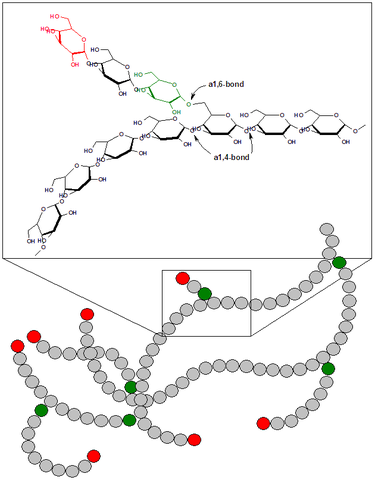
\includegraphics{figures/Glycogen.png}
\caption{The structure of glycogen.  Note the location of branch points ($\alpha$1-6 glycosidic linkages in green) and reducing ends (red) From \url{https://commons.wikimedia.org/w/index.php?curid=611992.}}
\label{fig:glycogen-structure}
\end{marginfigure}

\newthought{Because branch points need to be removed by a separate enzyme\sidenote{known as glycogen debranching enzyme or amylo-alpha-1, 6-glucosidase (encoded by the \textit{AGL} gene).},} overly branched glycogen is extremely compact, but its digestion may be limited by how well Glycogen Phosphorylase and the glycogen debranching enzyme can work in concert.  Defects in debranching enzyme result in a glycogen storage disease characterized by an inability to eliminate these branch points (see the section on Glycogen storage diseases below).

\subsection{Different tissues use glycogen for different purposes}

Glycogen is an easily accessible source of glucose for many tissues.  The content of glycogen ranges from 1-3\% of total weight in muscle tissue to up to 10\% of total mass in a well fed liver.  Since glycogen is very hydrophilic, it is estimated that approximately 3g of water are bound for every gram of glycogen \citep{Olsson1970,Fernandez-Elias2015}.  This is one reason why very low carbohydrate diets can result in rapid, initial weight loss, as glycogen is rapidly depleted. Based on what we have already learned about how glucose and phosphorylation differs between cells, different tissues use glycogen for slightly different reasons.  In general, muscle cells use glycogen when energy is needed, for example during exercise.  Liver cells on the other hand store glycogen to make glucose available for itself and other tissues, rather than for energy.

\newthought{Glycogen is an important energy source.}   Muscle tissue can have dramatic and rapid depletions of ATP in response to exercise.  The initial resource to replenish ATP is the creatine phosphate system described in Figure \ref{fig:creatine-kinase}.  Think of creatine phosphate like the battery on your laptop, and can supply (or store) excess ATP\sidenote{We will discuss this in the unit on non-protein compounds derived from amino acids later in the semester.}/  The amount of creatine phosphate can be quickly depleted, so muscle cells next turn to glycogen for glucose.  These glucose molecules typically undergo glycolysis (and depending on the fiber type) then the TCA cycle and electron transport chain to make ATP\sidenote{Recall, the absence of glucose-6-phosphatase means that liberated glucose-6-phosphate will not be dephosphoryated for extracellular release.}. As we will describe below, the primary signals for glycogen metabolism in muscle are energy dependent.

\begin{marginfigure}
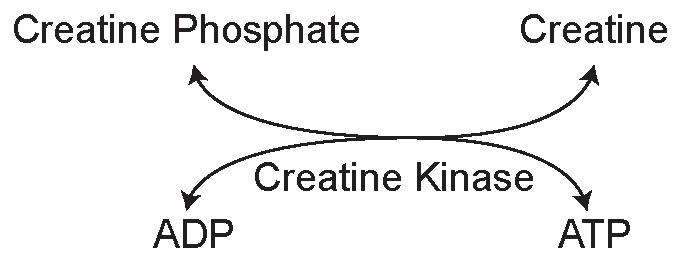
\includegraphics{figures/creatine-kinase.pdf}
\caption{The creatine phosphate system.  When ATP levels are depleted, the first reserve is creatine phosphate, which can transfer its high-energy phosphate group to ATP.  In times of plenty, creatine phosphate can be regenerated from excess ATP.  Muscle has large amounts of the enzyme that catalyzes this reaction, Creatine Kinase}
\label{fig:creatine-kinase}
\end{marginfigure}

\newthought{Glycogen plays an important role in endurance exercise.}  During prolonged exercise, muscle glycogen can be dramatically depleted.  To prevent this, athletes often ingest carbohydrates during exercise in order to continuously provide energy to the contracting muscles.  Another approach is to deplete glycogen levels prior to exercise, then eat a large carbohydrate rich meal.  This results in \emph{more} glycogen storage than the normal fed states, a condition known as glycogen super-compensation.  These extra glycogen stores are thought to fuel a longer sustained effort during exercise\sidenote{If you are interested in exploring this more, consider the bonus group assignment Glycogen Stores and Sports Nutrition, or doing a research project on this topic.}.  For more information on this concept see \citet{Hawley1997}.  

\newthought{Glycogen from the liver plays an important role in glucose homeostasis.}  The liver on the other hand mobilizes glycogen in order to maintain glucose levels in blood.  Whether due to fasting, or exercise the body needs to make glucose available for many tissues.  This is especially important for the brain, which is very poor at converting fatty acids into ATP.  As such, glycogen levels in the liver are generally controlled by indicators of glucose levels, such as glucose-6-phosphate.  Unlike the muscle, once glycogen is catabolized into glucose-6-phosphate it can be dephosporylated and released from hepatocytes for transport to other tissues.

\section{Regulation of glycogen synthesis}

Glycogen is stored when glucose and energy are plentiful.  After a typical meal, in a healthy person glycogen levels increase by about 50\% peaking about 4h after a meal \citep{Taylor1996a}.  This is due to a combination of increased glucose availability and the postprandial actions of insulin.  Glycogen is synthesized starting from Glucose-6-phosphate via the following series of reactions:

\begin{equation}
Glucose-6-phosphate \rightleftharpoons Glucose-1-phosphate
\end{equation}

\begin{equation}
Glucose-1-phosphate + UTP \rightleftharpoons UDP-Glucose + PPi
\end{equation}

\begin{equation}
UDP-Glucose + Glycogen_n \rightarrow Glycogen_{n+1}
\end{equation}

There are two important things to note about this process, one is that the first two reversible steps mean that the levels of G6P are extremely important in this process\sidenote{Recall from the lecture on glycolysis that G6P levels are controlled by the levels of glucose in the cell, the activity of hexokinase/glucokinase and the activity of PFK1, the rate limiting step in glycolysis.}.  The second is that by using UTP to activate glucose, this is an \emph{energy consuming process}.  This means that there is an energetic cost (the equivalent of one ATP phosphodiester bond) to storing glycogen\sidenote{Put another way, this means that to store and then release 1000 molecules of glycogen, you will use up the equivalent of 1000 ATP molecules.  In the end, you have used up 1000 ATP molecules but end up where you started, with available glucose.  This is another example of metabolic inefficiency, and is measured as part of the energy released during diet-induced thermogenesis.}.  The third reaction is catalyzed by the enzyme Glycogen Synthase\sidenote{There are two isoforms of Glycogen Synthase, one expressed in muscle and brain (\textit{GYS1}) and one expressed in the liver and fat, encoded by the \textit{GYS2} gene.} and that is the main point of regulatory control in glycogen synthesis.

\subsection{Glycogen Synthase is activated by Glucose-6-phosphate}

Both isoforms of Glycogen Synthase are allosterically activated by glucose-6-phosphate as first described in the late 1950s by \citet{Leloir1959}.  G6P levels are increased when glycolysis is low, but glucose levels are high.  This is generally a situation where nutrient levels are high, but energy demand is low.  This is a good time to store extra glucose, so this makes physiological sense.

\begin{table}
\centering
\caption{Protein kinases that phosphorylate and inactivate Glycogen Synthase.}
\label{tab:gs-sites}
\begin{tabular}{cc}
\hline
\textbf {Kinase} & \textbf{Signal}  \\
\hline
PKA & Adrenaline/Glucagon \\
GSK3 & Insulin (inactivates) \\
AMPK & Energy Stress \\
\hline
\end{tabular}
\end{table}

\subsection{Extracellular control and signaling}

In addition to this metabolite-level control, Glycogen Synthase is also regulated by reversible protein phosphorylation \citep{Larner1960}\sidenote{This was one of the earliest described examples of metabolic control by protein phosphorylation.}.  There are several protein kinases that regulate Glycogen Synthase, and as a general rule they result in the \emph{inactivation} of the enzyme.  These kinases are summarized in Table \ref{tab:gs-sites}.  Insulin \emph{activates} Glycogen Synthase, and it does so by \emph{dephosphorylating} these sites (see Figure \ref{fig:glycogen-phosphorylation}).  Part of this mechanism is by reducing the activity of the kinases (especially GSK3 and PKA) but insulin also functions by activating protein phosphatase activity towards Glycogen Synthase.  This is accomplished via a series of proteins that specifically target a protein phosphatase on the glycogen particle.  The precise mechanisms by which insulin promotes this dephosphorylation are still unclear.  At the same time that Glycogen Synthase is being dephosphorylated (and activated), Glycogen Phosphorylase\sidenote{The enzyme that cleaves glucose from an existing glycogen molecule} is also dephosphorylated and inactivated.

\begin{figure}
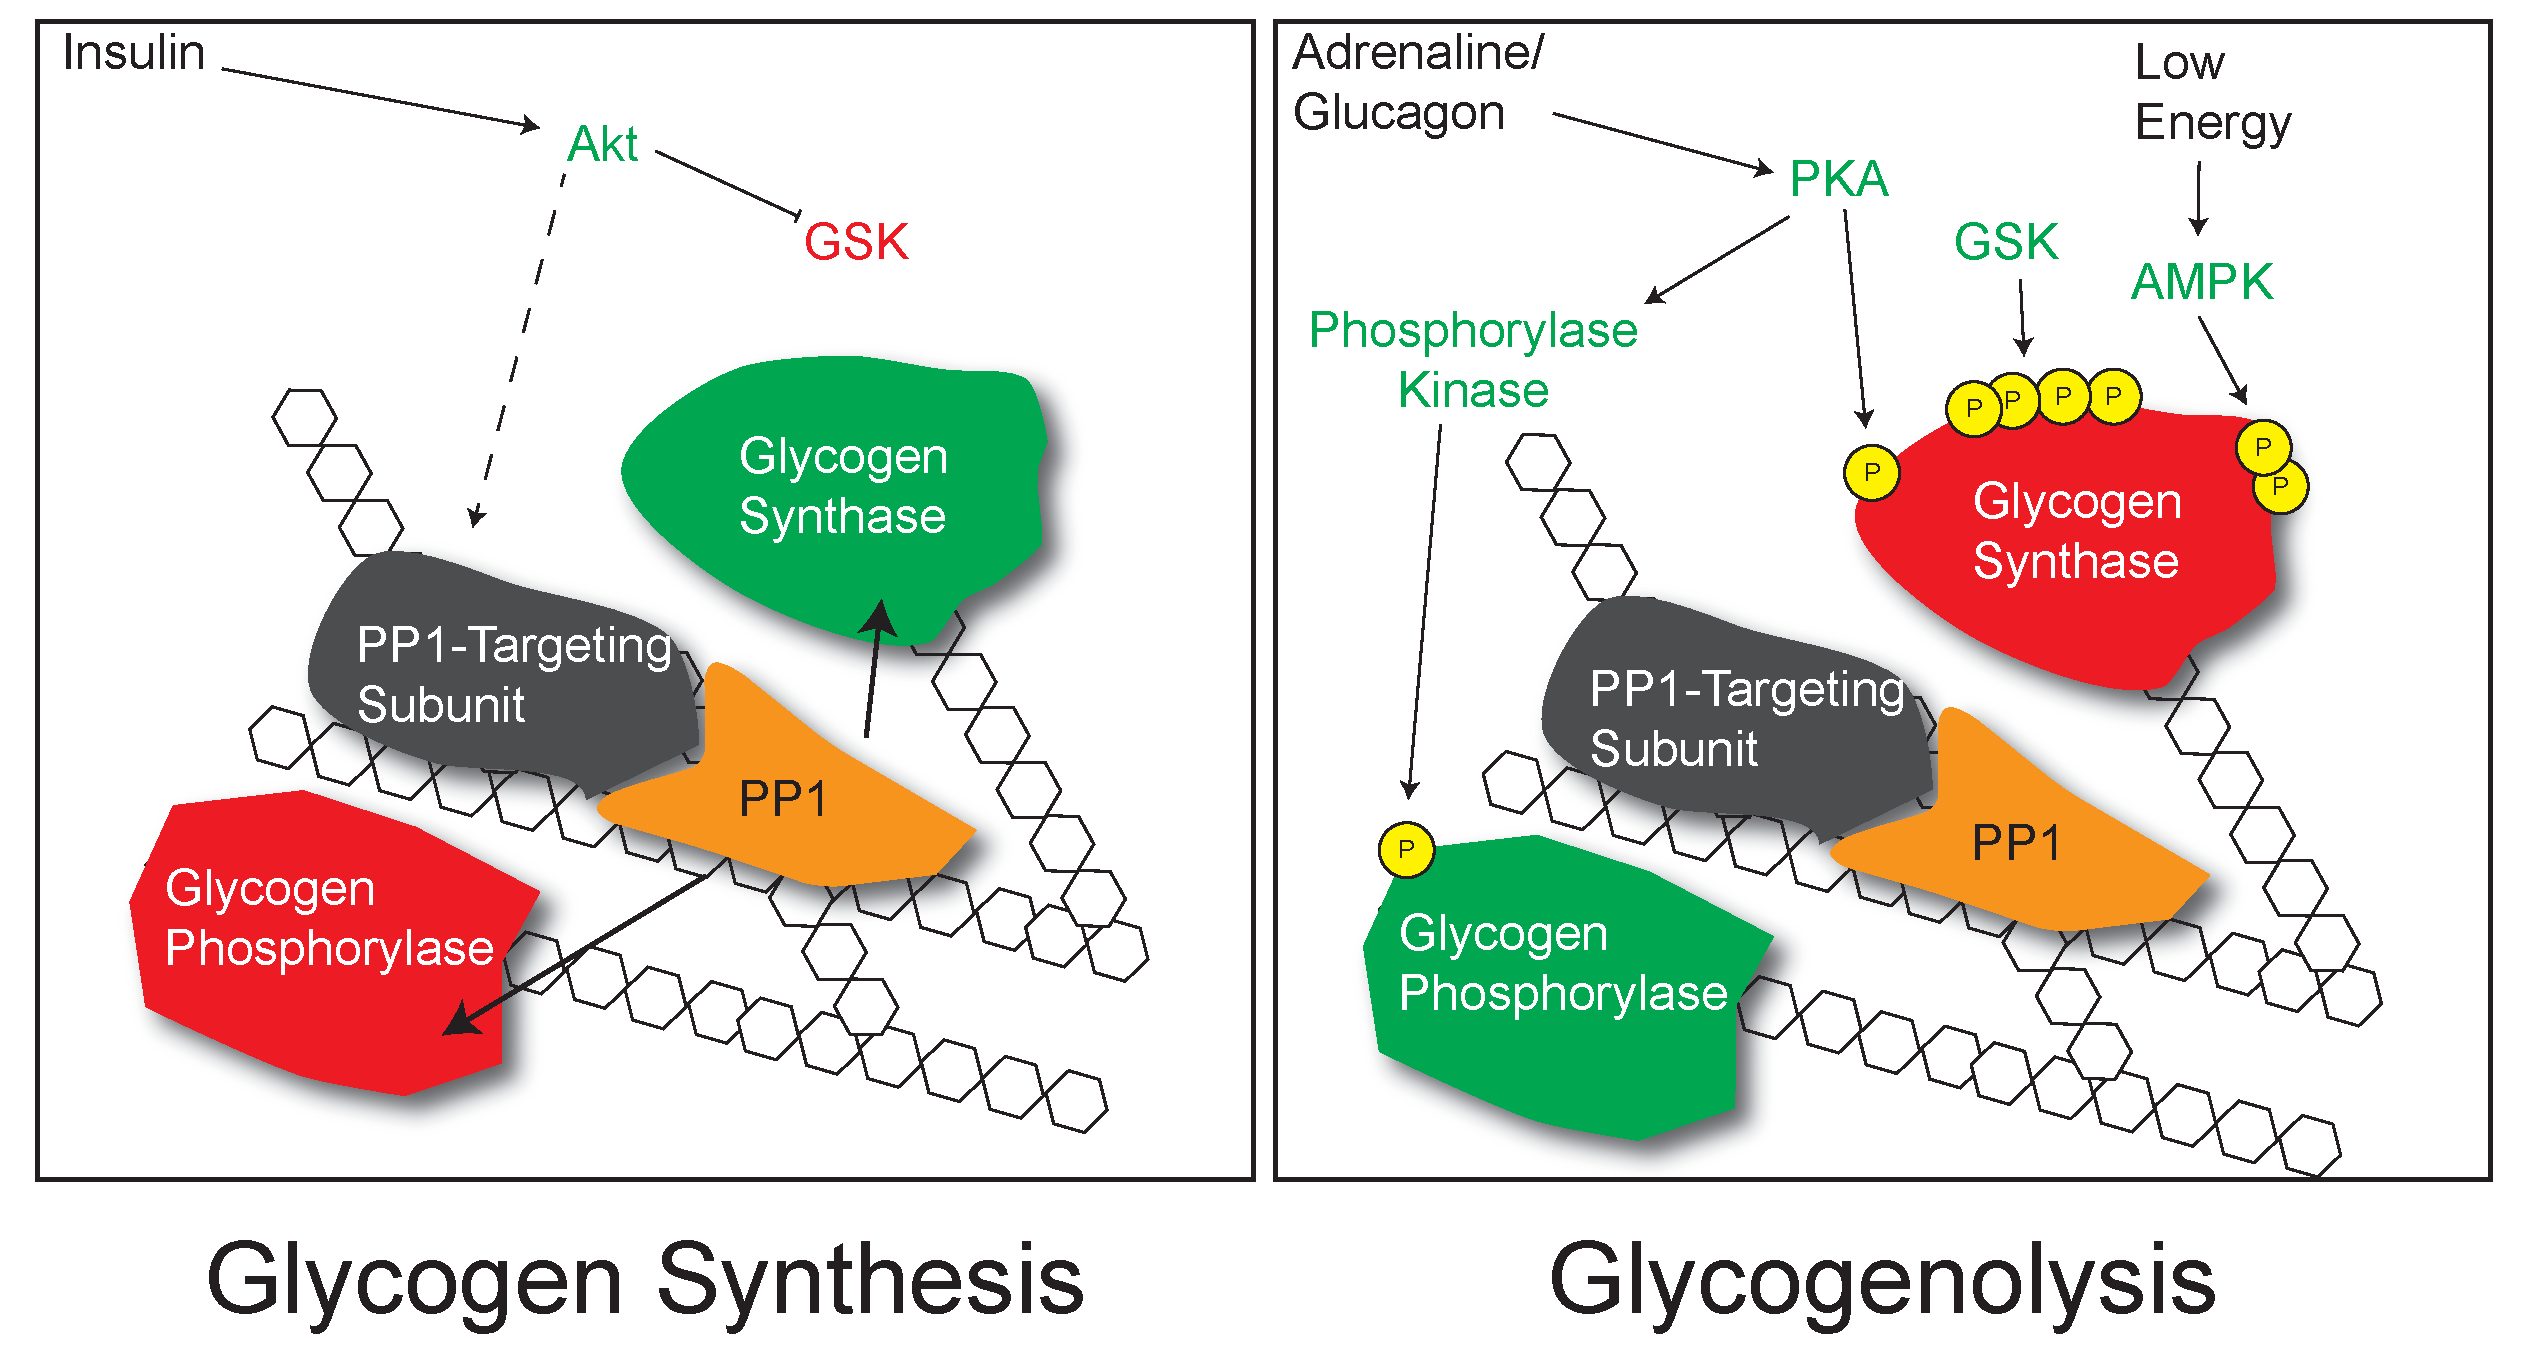
\includegraphics{figures/glycogen-phosphorylation}
\caption{Post-translational regulation of glycogen metabolism.  Red indicates inactive enzymes, while green indicates active enzymes. PP1 is a protein phosphatase that removes the phosphate groups from both Glycogen Synthase and Glycogen Phosphorylase.  The dashed arrow indicates the mechanisms by which this phosphatase are activated are currently unknown.}
\label{fig:glycogen-phosphorylation}
\end{figure}

\newthought{Separate from the effects of insulin on Glycogen Synthase activity,} recall that insulin will also promote glucose uptake (in muscle and fat tissues).  This increased glucose flux will result in more Glucose-6-phosphate in the cell and allosteric activation of Glycogen Synthase.  Therefore there are at least two ways by which insulin can promote glycogenesis.

\section{Regulation of glycogen breakdown}

Glycogen is broken down to release glucose in two steps\sidenote{This mechanism is specific to the $\alpha$(1-4) linkages, not the branch points, which will be described later.}:

\begin{equation}
Glycogen_{n} \rightarrow Glycogen_{n-1} + Glucose-1-phosphate
\end{equation}

\begin{equation}
Glucose-1-phosphate \leftrightarrow Glucose-6-phosphate
\end{equation}

The fate of Glucose-6-phosphate depends on the relative activities of PFK1, Glucose-6-phosphate dehydrogenase\sidenote{Leading towards the pentose phosphate pathway.} and, in the case of liver cells Glucose-6-phosphatase.  Generally, in the muscle the liberated Glucose-6-phosphate enters glycolysis wheras in the liver it is dephosphorylated and released as glucose.

\subsection{Intracellular control}

The first, and rate limiting step of glycogenolysis is catalyzed by an enzyme named Glycogen Phosphorylase\sidenote{There are three isoforms of this gene, \textit{PYGL}, \textit{PYGM} and \textit{PYGB} which are expressed in the liver, muscle and brain respectively.}.  Glycogen Phosphorylase is allosterically activated by AMP.  This activation by AMP is blocked by the presence of ATP or Glucose-6-phosphate.  AMP is increased when there is energy demand, so if there is a need for energy, Glycogen Phosphorylase gets activated.  This can be over-ridden when ATP is plentiful (indicating a lack of energy stress) or Glucose-6-phosphate is elevated (indicating sufficient glucose levels).  While all three isoforms respond similarly in direction, the muscle enzyme is much more sensitive to activation by AMP than the liver enzyme.  This is due to structural differences in the AMP-binding pocket between the muscle and liver isoforms \citep{Rath2000}.  As part of its reaction mechanism, Glycogen Phosphorylase also uses Vitamin B$_6$-derived Pyridoxal phosphate as a prosthetic group\sidenote{Vitamin B$_6$ has many other roles, but has been shown to be effective in treating McArdle's disease, a genetic deficiency in \textit{PYGM}.}.

\begin{marginfigure}
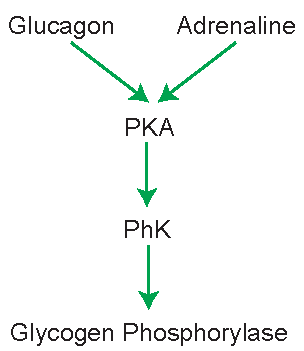
\includegraphics{figures/gp-activation.pdf}
\caption{Hormonal regulation of glycogen phosphorylase through PKA and Phosphorylase Kinase (PhK).}
\label{fig:gp-activation}
\end{marginfigure}

\subsection{Extracellular control and signaling}

The activation of Glycogen Phosphorylase by AMP can be over-ridden by protein phosphorylation by an enzyme named Phosphorylase Kinase (see Figure \ref{fig:gp-activation}).  Once phosphorylated, the enzyme functions as if it is in the AMP-activated state.  The phosphorylation of Glycogen Phosphorylase is activated by PKA dependent signaling, induced by either glucagon in the liver or adrenaline in liver, muscle and other tissues.  Similarly, PKA-dependent signaling phosphorylates and inactivates Glycogen synthase.  This means that adrenergic signaling turns Glycogen Phosphorylase on, and Glycogen Synthase off simultaneously\sidenote{Also, insulin turns Glycogen Phosphorylase off, and Glycogen Synthase on.}.  A summary of the effects of reversible protein phosphorylation on the enzymes of glycogen metabolism is shown in Table \ref{tab:gs-gp-phosphorylation}.

\subsection{Regulation of glycogen branching and removal of branch points}

The generation and removal of glycogen branch points is an important part of glycogen metabolism.  Glycogen Phosphorylase can only cleave at $\alpha$1-4 bonds and cannot proceed past $\alpha$1-6 linkages.  Whenever a $\alpha$1-6 linkage is encountered, the Glycogen Debranching Enzyme is recruited, which removes the $\alpha$1-6 link and allows for Glycogen Phosphorylase to proceed.  Currently, there is no strong data suggesting that either Glycogen Branching or Debranching Enzymes are regulated by metabolites, or hormonal signals, but inappropriate activity can result in under- or over-branched glycogen.


\begin{table}
\centering
\caption{Summary of how protein phosphorylation regulates Glycogen Synthase and Glycogen Phosphorylase.}
\label{tab:gs-gp-phosphorylation}
\begin{tabular}{cc}
\hline
\textbf {Enzyme} & \textbf{Effects of Phosphorylation}  \\
\hline
Glycogen Synthase & Inactivates - Less Synthesis \\
Glycogen Phosphorylase & Activates - More Breakdown\\
\hline
\end{tabular}
\end{table}

\section{Glycogen storage diseases}

There are a variety of rare, heritable defects which result in abberant glycogen metabolism (see Table \ref{tab:glycogen-storage-diseases}).  Some of these result in an inability to synthesize glycogen, while others prevent glycogenolysis, resulting in pathologically large particles of glycogen resulting in cell death.  Some common glycogen storage diseases, and the affected enzyme are below.   

\begin{table}
\centering
\caption{Some example glycogen storage diseases and the gene that is mutated.  \textit{G6PC}: Glucose-6-phosphatase; \textit{PFKM}: Muscle PFK1; \textit{PHKA1/2}: Phosphorylase kinase; \textit{SLC4A2}: GLUT2.  Before class, try to predict what the loss of activity of these proteins would do to glycogen levels.}.
\label{tab:glycogen-storage-diseases}
\begin{tabular}{ccc}
\hline
\textbf {Disease} & \textbf{Enzyme} & \textbf{Predicted Glycogen Levels} \\
\hline
Fanconi-Bickel syndrome & \textit{SLC4A2} & \\
von Gierke's disease & \textit{G6PC} & \\
Tarui's disease & \textit{PFKM} & \\
GSD Type 0 & \textit{GYS2} & \\
Cori's disease & \textit{AGL} & \\
Andersen disease & \textit{GBE} & \\
McArdle disease& \textit{PYGM} & \\
Hers' disease & \textit{PYGL} & \\
GSD type IX & \textit{PHKA1/2} & \\
\hline
\end{tabular}
\end{table}


\bibliography{library}
\bibliographystyle{plainnat}

\end{document}
